\documentclass[11pt,a4paper]{article}

\usepackage[margin=2.5cm]{geometry}
\usepackage[T1]{fontenc}
\usepackage[utf8]{inputenc}
\usepackage{amsmath}
\usepackage{amssymb}
\usepackage{booktabs}
\usepackage{graphicx}
\usepackage{subcaption}
\usepackage{float}
\usepackage{hyperref}
\usepackage{url}
\usepackage{microtype}

\hypersetup{
  colorlinks=true,
  linkcolor=blue,
  citecolor=blue,
  urlcolor=blue
}

\title{Project III: Generative Models for Cat Image Synthesis}
\author{Michał Pytel, Sebastian Trojan}
\date{\today}

\begin{document}
\maketitle

\begin{abstract}
This report compares three generative modelling approaches for $64\times64$ cat image synthesis:
a Deep Convolutional Generative Adversarial Network (DCGAN), a residual convolutional variational autoencoder (VAE), and a compact denoising diffusion probabilistic model (DDPM).
All input images were centre-cropped to square format, resized to $64\times64$, and normalised to $[-1,1]$. The models were trained under a limited-compute setup.
Within each model family, selected hyperparameters were varied and evaluated using Fr\'echet Inception Distance (FID), lightweight diversity diagnostics, qualitative sample grids, and latent/noise interpolation.
The strongest cat-only results were obtained by the wider DDPM, followed by the best DCGAN variant and then the best VAE variant. Because DDPM FID was computed with fewer generated samples, the final ranking is interpreted together with visual inspection.
An exploratory cats-and-dogs extension was also trained to examine how unconditional models behave on a mixed animal distribution.
\end{abstract}

\clearpage
\tableofcontents
\clearpage

\section{Introduction}

Generative image modelling is the task of learning a data distribution well enough to create new, previously unseen samples from it.
Cat photographs are a useful test case because they contain a recognisable semantic object, but still vary strongly in pose, colour, background, crop, lighting, and resolution.
This makes the task more informative than generating simple synthetic patterns, while still small enough to study with limited computing resources.

This project investigates three representative families of generative models: a Deep Convolutional Generative Adversarial Network (DCGAN), a variational autoencoder, and a denoising diffusion model.
The aim is not to reproduce state-of-the-art large-scale image generation, but to build a controlled and reproducible comparison of methods that can be trained locally.
All models are therefore trained at $64\times64$ resolution, with compact architectures and a small set of targeted hyperparameter experiments.

The comparison uses both quantitative and qualitative evidence.
Fr\'echet Inception Distance (FID) is used to compare generated and real image distributions, while sample grids, VAE reconstructions, interpolation grids, and lightweight diversity statistics are used to inspect failure modes that a single number may hide.
Because GANs are prone to mode collapse, DCGAN samples are additionally checked for repeated poses, colours, textures, and low diversity.
The project also includes an exploratory extension in which the best cat-only configurations are trained on a mixed cats-and-dogs dataset to observe how unconditional models handle a multi-class distribution.

\section{Literature review}

\subsection{Variational Autoencoders}

A VAE \cite{kingma2014vae} couples an encoder $q_\phi(\mathbf{z}\mid\mathbf{x})$ and a decoder $p_\theta(\mathbf{x}\mid\mathbf{z})$. In this project it is described using the following $\beta$-weighted objective, which reduces to the standard evidence lower bound when $\beta=1$:
\begin{equation}
  \mathcal{L}_{\text{ELBO}} =
  \mathbb{E}_{q_\phi(\mathbf{z}\mid\mathbf{x})}\big[\log p_\theta(\mathbf{x}\mid\mathbf{z})\big]
  - \beta\,\mathrm{KL}\!\big(q_\phi(\mathbf{z}\mid\mathbf{x}) \,\|\, p(\mathbf{z})\big),
\end{equation}
where $p(\mathbf{z})=\mathcal{N}(0,I)$ and $\beta$ trades reconstruction against latent regularisation.
The standard VAE \cite{kingma2014vae} corresponds to $\beta=1$. The explicit weighting parameter was introduced later by the $\beta$-VAE \cite{higgins2017betavae} and is used here to make the reconstruction--prior trade-off visible.
VAEs give a continuous, interpolable latent space, which is convenient for the interpolation task, but their pixel-wise reconstruction objective typically yields blurry samples.
The vector-quantised variant VQ-VAE \cite{vandenoord2017vqvae} and its successor VQ-VAE-2 \cite{razavi2019vqvae2} replace the continuous latent with a discrete codebook to sharpen outputs.

\subsection{Generative Adversarial Networks}

A GAN \cite{goodfellow2014gan} trains a generator $G$ and discriminator $D$ in a minimax game:
\begin{equation}
  \min_G \max_D
  \mathbb{E}_{\mathbf{x}\sim p_{\text{data}}}[\log D(\mathbf{x})]
  + \mathbb{E}_{\mathbf{z}\sim p(\mathbf{z})}[\log(1 - D(G(\mathbf{z})))].
\end{equation}
DCGAN \cite{radford2016dcgan} established the convolutional recipe of strided/transposed convolutions, batch normalisation, and fully convolutional design.
GAN training is notoriously unstable. Common stabilisers include spectral normalisation of the discriminator \cite{miyato2018spectralnorm}, the Wasserstein GAN \cite{arjovsky2017wgan} and WGAN-GP \cite{gulrajani2017wgangp}, and adaptive discriminator augmentation (ADA) \cite{karras2020ada}, which helps prevent discriminator overfitting when data is scarce.
StyleGAN2 \cite{karras2020stylegan2} represents the high-fidelity end of this family but is heavier than the compute budget of this project.

\subsection{Diffusion Models}

Diffusion models \cite{sohldickstein2015} define a forward process that gradually adds Gaussian noise over $T$ steps and learn a network to reverse it.
DDPM \cite{ho2020ddpm} showed that a simple noise-prediction objective,
\begin{equation}
  \mathcal{L}_{\text{simple}} =
  \mathbb{E}_{t,\mathbf{x}_0,\boldsymbol{\epsilon}}
  \Big[\,\big\|\boldsymbol{\epsilon} - \boldsymbol{\epsilon}_\theta(\mathbf{x}_t, t)\big\|^2\,\Big],
  \quad
  \mathbf{x}_t = \sqrt{\bar\alpha_t}\,\mathbf{x}_0 + \sqrt{1-\bar\alpha_t}\,\boldsymbol{\epsilon},
\end{equation}
yields high-quality images.
Improved DDPM \cite{nichol2021improved} added learned variances and a cosine noise schedule. ADM \cite{dhariwal2021beatsgans} demonstrated that diffusion can surpass GANs on FID.
DDIM \cite{song2021ddim} introduced a deterministic, non-Markovian sampler that both accelerates sampling and defines a useful mapping from an initial noise tensor to an image.
Latent Diffusion \cite{rombach2022ldm} moves the process into a learned latent space for efficiency. It is noted as context but not used here.

\subsection{Evaluation: Fr\'echet Inception Distance}

FID \cite{heusel2017fid} compares the statistics of Inception-V3 features of real and generated images, modelling each as a multivariate Gaussian:
\begin{equation}
  \mathrm{FID} =
  \|\mu_r - \mu_g\|_2^2
  + \mathrm{Tr}\!\Big(\Sigma_r + \Sigma_g - 2(\Sigma_r \Sigma_g)^{1/2}\Big),
\end{equation}
where $(\mu_r, \Sigma_r)$ and $(\mu_g, \Sigma_g)$ are the feature means and covariances of real and generated sets.
Lower FID is better.
FID is sensitive to sample count. Therefore, the sample count is reported wherever FID results are discussed.

\section{Dataset and preprocessing}

The cat dataset contains 9997 images \cite{catdataset}.
The exploratory mixed dataset uses the Kaggle Dogs vs.\ Cats data \cite{dogsvscats} and contains 25000 training images.
The raw images have different resolutions and aspect ratios, so each image was:
\begin{enumerate}
  \item converted to RGB,
  \item centre-cropped to a square using the shorter side,
  \item resized to $64\times64$ using bicubic interpolation,
  \item randomly horizontally flipped during training,
  \item normalised to $[-1,1]$.
\end{enumerate}
Using $64\times64$ resolution was a deliberate compute-saving decision: it allowed all three model families and multiple hyperparameter variants to be trained and evaluated on a consumer GPU.

\section{Methods}

This section describes the baseline configuration for each model family.
The later hyperparameter study changes one main factor at a time from these baselines and then selects the best-performing variant for final comparison.

\subsection{VAE}

The VAE is a residual convolutional model with GroupNorm, SiLU activations, attention at low resolution, and a global Gaussian latent vector.
The baseline VAE uses latent dimension 384, base channel count 64, channel multipliers $(1,2,4,8)$, dropout 0.03, and one decoder refinement block.
It is trained for 300 epochs with batch size 64, Adam learning rate $1.5\cdot10^{-4}$, weight decay $10^{-6}$, gradient clipping at 1.0, and mixed precision.
The baseline KL weight is warmed up from 0 to $\beta=0.18$ over 60 epochs, with free bits set to 0.005.
The reconstruction term combines MSE and L1 losses, and the final loss is:
\begin{equation}
  \mathcal{L}_{\text{VAE}} =
  \mathcal{L}_{\text{recon}} + \beta \mathcal{L}_{\text{KL}}.
\end{equation}
The baseline reconstruction objective uses MSE weight 1.0, L1 weight 0.25, and a two-level multiscale term with weight 0.5.
Although the baseline configuration uses temperature 0.75 for periodic training samples, final VAE evaluation sweeps temperatures 0.50, 0.65, and 0.80 because sampling temperature strongly affects random generations.

\subsection{DCGAN}

The DCGAN uses a convolutional generator and discriminator trained with least-squares GAN loss.
The baseline uses latent vector dimension 100, generator feature width 64, discriminator feature width 64, batch size 128, and 300 training epochs.
It is trained with Adam using generator learning rate $2\cdot10^{-4}$, discriminator learning rate $5\cdot10^{-5}$, $\beta_1=0.5$, and $\beta_2=0.999$.
Label smoothing sets the real target to 0.9.
Small instance noise with initial standard deviation 0.02 is added and decayed over 50 epochs.
Generator and discriminator gradients are clipped at 5.0.
The baseline does not use minibatch-standard-deviation features, discriminator dropout, or mixed precision.

\subsection{DDPM}

The DDPM uses a compact U-Net denoiser with residual blocks, attention at $16\times16$ resolution, and 500 diffusion timesteps.
The baseline U-Net uses base channel count 64, channel multipliers $(1,2,4,4)$, two residual blocks per resolution level, dropout 0.1, and attention at $16\times16$.
The baseline diffusion process uses 500 timesteps with a linear beta schedule from $10^{-4}$ to 0.02.
It is trained for 300 epochs with batch size 32, Adam learning rate $2\cdot10^{-4}$, no weight decay, gradient clipping at 1.0, and mixed precision.
Generation starts from Gaussian noise and iteratively denoises it into an image.
This iterative sampling is slower than GAN/VAE generation, so DDPM FID is computed with fewer generated samples than DCGAN and VAE.

\section{Hyperparameter studies}

Each model family was compared internally by changing one main factor at a time.
All variants were trained from scratch for 300 epochs.
During training, sample grids were saved every 5 epochs and checkpoints every 10 epochs.
The latest checkpoint of each run was then evaluated with FID and visually inspected.
DCGAN and VAE FID used 5000 generated images.
DDPM FID used 2500 generated images because DDPM sampling requires hundreds of denoising steps per image.
Lower FID indicates that generated images are closer to the real-image feature distribution.
Because FID is sample-count sensitive, values are most directly comparable within a model family.
Cross-family comparisons involving DDPM should be read together with the qualitative grids.

\subsection{DCGAN experiments}

The DCGAN sweep tested whether image quality was limited more by generator capacity, discriminator strength, or stabilisation choices.
Starting from the baseline, the following changes were evaluated separately: increasing discriminator learning rate, reducing generator learning rate, increasing latent dimensionality to 128, widening the generator to feature width 96, removing instance noise, removing label smoothing, and adding minibatch-standard-deviation features.
\begin{table}[H]
\centering
\caption{DCGAN hyperparameter comparison.}
\label{tab:dcgan-hparam}
\begin{tabular}{llr}
\toprule
Variant & Main change & FID \\
\midrule
Stronger discriminator & discriminator LR $=10^{-4}$ & \textbf{143.79} \\
Larger generator & generator feature width 96 & 153.95 \\
No instance noise & removed input noise & 155.60 \\
Baseline & reference setting & 161.62 \\
Larger latent vector & latent dim 128 & 172.66 \\
No label smoothing & real label target 1.0 & 173.37 \\
Lower generator LR & generator LR $=10^{-4}$ & 175.31 \\
Minibatch standard deviation & extra diversity feature & 183.10 \\
\bottomrule
\end{tabular}
\end{table}

The best DCGAN result came from increasing the discriminator learning rate while keeping the other stabilisers active. This suggests that the baseline generator benefited from a slightly stronger discriminator signal, but only when label smoothing and instance noise were still used.

\subsection{VAE experiments}

The VAE sweep focused on the reconstruction--prior trade-off.
The baseline was compared with intermediate and stronger KL regularisation, a prior-matching variant, larger and smaller latent dimensions, an extra decoder refinement block, and removal of the multiscale reconstruction term.
Because random VAE samples depend strongly on how widely the Gaussian prior is sampled, each VAE checkpoint was evaluated at temperatures 0.50, 0.65, and 0.80.
Table \ref{tab:vae-hparam} reports only the best temperature for each variant, while the complete temperature grid is reported in Appendix \ref{app:vae-full-results}.

\begin{table}[H]
\centering
\caption{VAE hyperparameter comparison using the best sampling temperature found for each variant.}
\label{tab:vae-hparam}
\begin{tabular}{llrr}
\toprule
Variant & Main change & Best temp. & Best FID \\
\midrule
$\beta=0.5$ & stronger KL regularisation & 0.65 & \textbf{176.68} \\
Prior-matching variant & stronger prior matching & 0.50 & 189.33 \\
$\beta=0.25$ & intermediate KL regularisation & 0.50 & 191.54 \\
Extra decoder refinement & extra decoder refine block & 0.50 & 193.75 \\
No multiscale loss & single-scale reconstruction & 0.50 & 199.47 \\
Latent dimension 512 & larger latent space & 0.65 & 224.25 \\
Latent dimension 256 & smaller latent space & 0.65 & 226.71 \\
Baseline & reference setting & 0.65 & 241.81 \\
\bottomrule
\end{tabular}
\end{table}

\begin{table}[H]
\centering
\caption{VAE sampling-temperature summary across all eight VAE variants. The standard deviation is computed across variants at the same temperature.}
\label{tab:vae-temp-summary}
\begin{tabular}{rrr}
\toprule
Temperature & Mean FID $\pm$ std. & Best FID \\
\midrule
0.50 & \textbf{209.25 $\pm$ 24.10} & 188.23 \\
0.65 & 209.89 $\pm$ 20.78 & \textbf{176.68} \\
0.80 & 230.99 $\pm$ 14.74 & 199.93 \\
\bottomrule
\end{tabular}
\end{table}

In Table \ref{tab:vae-temp-summary}, boldface marks the best value in each column.
This distinction is important because temperature 0.50 gives the best average behaviour across VAE variants, whereas temperature 0.65 gives the best single VAE result.

\begin{figure}[H]
\centering
\begin{subfigure}{0.32\linewidth}
  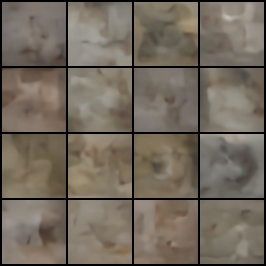
\includegraphics[width=\linewidth]{report_figures/vae_temperature_050.png}
  \caption{Temperature 0.50}
\end{subfigure}
\begin{subfigure}{0.32\linewidth}
  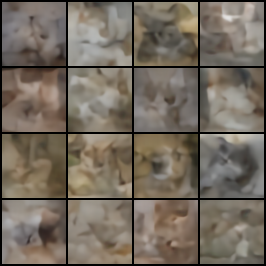
\includegraphics[width=\linewidth]{report_figures/vae_temperature_065.png}
  \caption{Temperature 0.65}
\end{subfigure}
\begin{subfigure}{0.32\linewidth}
  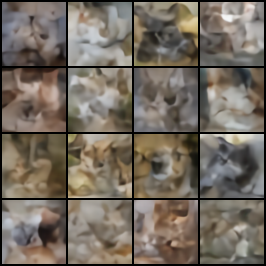
\includegraphics[width=\linewidth]{report_figures/vae_temperature_080.png}
  \caption{Temperature 0.80}
\end{subfigure}
\caption{Side-by-side VAE samples for the $\beta=0.5$ model at three sampling temperatures. The same random seed was used in each case, so the comparison isolates the effect of scaling the latent prior sample.}
\label{fig:vae-temperature}
\end{figure}

Figure \ref{fig:vae-temperature} illustrates the sampling-temperature trade-off for the selected VAE.
At temperature $0.50$, samples are more conservative and smoother, but diversity is reduced.
At temperature $0.80$, the latent samples explore a wider region of the prior, which increases variation but also introduces more malformed textures.
Across all VAE variants, temperature $0.50$ has the best mean FID, but the best single VAE result is obtained by the $\beta=0.5$ model at temperature $0.65$.
This is why temperature $0.65$ is used for the final selected VAE.
The complete VAE temperature results are listed in Appendix \ref{app:vae-full-results}.

\subsection{DDPM experiments}

The DDPM sweep tested model capacity, noise scheduling, regularisation, learning rate, and diffusion-chain length.
The baseline linear-schedule model was compared with a cosine schedule, a wider U-Net with base channel count 96, a lower learning rate, no dropout, and a longer 1000-step diffusion process.
Although the 1000-step model uses a finer noising chain, it is also slower to sample and did not improve FID in this limited-compute setting.

\begin{table}[H]
\centering
\caption{DDPM hyperparameter comparison.}
\label{tab:ddpm-hparam}
\begin{tabular}{llr}
\toprule
Variant & Main change & FID \\
\midrule
Wider U-Net & base channels 96 & \textbf{48.00} \\
Baseline & reference setting & 48.90 \\
Cosine schedule & cosine noise schedule & 64.18 \\
Lower learning rate & learning rate $=10^{-4}$ & 70.61 \\
No dropout & dropout disabled & 89.29 \\
Longer diffusion chain & 1000 timesteps & 90.19 \\
\bottomrule
\end{tabular}
\end{table}

The best DDPM result came from increasing U-Net width. The baseline was already close to this result, while the cosine schedule, lower learning rate, disabled dropout, and longer diffusion chain all reduced performance in this setup.

\section{Main results}

\subsection{Quantitative comparison}

Table \ref{tab:best-models} compares the selected configuration from each method. DCGAN and VAE use 5000 generated images for FID, while DDPM uses 2500 generated images. Lower FID is better. Diversity RMSE is the average pairwise RMSE in pixel space, and pixel std. is the average per-pixel standard deviation across generated images. Higher diversity values indicate more pixel-space variation.

\begin{table}[H]
\centering
\caption{Selected configurations and evaluation metrics for the final comparison.}
\label{tab:best-models}
\begin{tabular}{llrrr}
\toprule
Method & Selected variant & FID & Diversity RMSE & Pixel std. \\
\midrule
DCGAN & discriminator LR $10^{-4}$ & 143.79 & 0.3682 & 0.2644 \\
VAE & $\beta=0.5$, temp. 0.65 & 176.68 & 0.1351 & 0.0966 \\
DDPM & base channels 96 & \textbf{48.00} & \textbf{0.4179} & \textbf{0.3084} \\
\bottomrule
\end{tabular}
\end{table}

The selected DDPM has by far the lowest reported FID and also the highest diversity diagnostics.
Since its FID uses fewer generated images than DCGAN and VAE, the exact numerical margin should not be treated as a perfectly controlled comparison. However, the gap is large and is supported by visual inspection.
The DCGAN produces sharper outputs than the VAE but has a noticeably higher FID than DDPM.
The VAE trains stably and reconstructs real images well, but its random samples are smooth and less realistic.
The diversity diagnostics did not indicate severe mode collapse for any selected model.

\subsection{Qualitative comparison}

\begin{figure}[H]
\centering
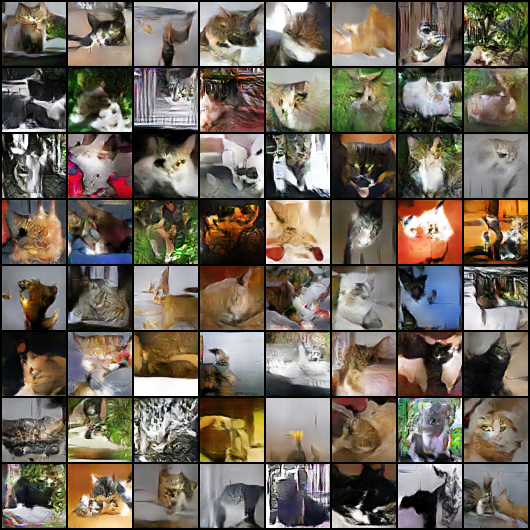
\includegraphics[width=0.72\linewidth]{report_figures/dcgan_samples.png}
\caption{Generated cat-only samples from DCGAN.}
\label{fig:dcgan-samples}
\end{figure}

\begin{figure}[H]
\centering
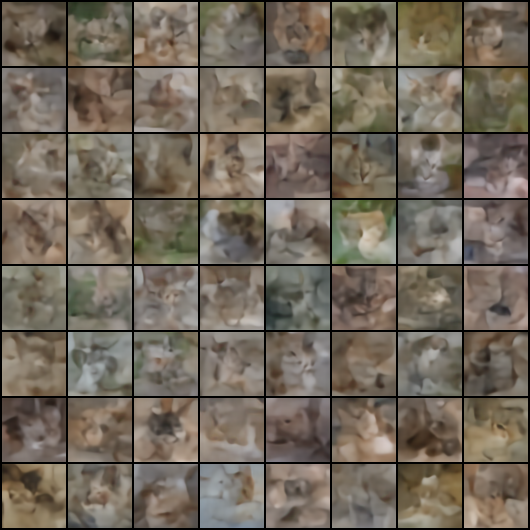
\includegraphics[width=0.72\linewidth]{report_figures/vae_samples.png}
\caption{Generated cat-only samples from VAE.}
\label{fig:vae-samples}
\end{figure}

\begin{figure}[H]
\centering
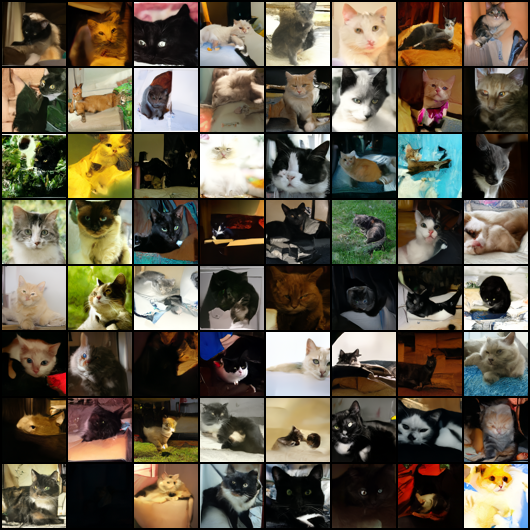
\includegraphics[width=0.72\linewidth]{report_figures/ddpm_samples.png}
\caption{Generated cat-only samples from DDPM.}
\label{fig:ddpm-samples}
\end{figure}

The DCGAN samples often contain recognisable cats, but many images have distorted anatomy or noisy local textures.
The VAE samples preserve broad colour and pose-like structure, but they are strongly blurred and often lack clear cat anatomy or fine detail.
The DDPM samples are the most convincing: many images show recognisable cat faces, fur colours, body poses, and diverse backgrounds.

The sample grids above describe random generation. The VAE also has an encoder, so it can be inspected through reconstructions of real validation images. Figure \ref{fig:vae-recon} shows this additional view of the VAE.

\begin{figure}[H]
\centering
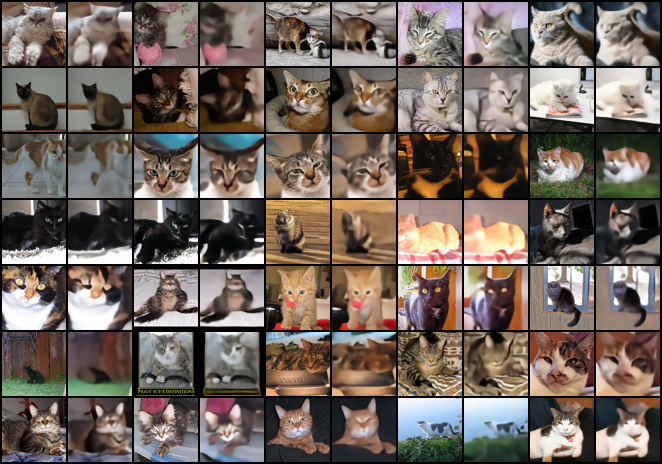
\includegraphics[width=0.9\linewidth]{report_figures/vae_reconstructions.png}
\caption{VAE reconstruction grid. Each pair shows a real image followed by its reconstruction.}
\label{fig:vae-recon}
\end{figure}

Figure \ref{fig:vae-recon} explains an important VAE behaviour.
The VAE reconstructs real cats reasonably well: pose and colour are preserved, but texture and edges are smoothed.
However, random VAE samples are much weaker than reconstructions because random generation samples from the prior $p(\mathbf{z})$, whereas reconstruction uses posterior latents inferred from real images.

\section{Mode collapse and diversity}

Mode collapse was assessed by visual sample grids and by simple pixel-space diversity diagnostics.
The diagnostics are not a substitute for distributional coverage metrics, but they are useful for detecting severe duplication or extremely low variation.
For the final selected models, the average pairwise RMSE values were $0.3682$ for DCGAN, $0.1351$ for VAE, and $0.4179$ for DDPM.
The lower VAE value is consistent with its blurry and visually similar random samples.
The DCGAN did not collapse to one image type, but the grid shows some repeated colour/texture patterns and malformed outputs.
The DDPM showed the highest measured diversity and the most varied samples.

If severe collapse had appeared in the DCGAN, the planned mitigations were label smoothing, instance noise, gradient clipping, rebalancing generator and discriminator learning rates, and minibatch-standard-deviation features.
In the tested sweep, minibatch standard deviation did not improve FID. The best DCGAN used a moderately stronger discriminator learning rate together with label smoothing and instance noise.

\section{Interpolation}

For each selected model, two latent/noise tensors were sampled and linearly interpolated into 10 total points:
\[
  \mathbf{z}_\alpha = (1-\alpha)\mathbf{z}_0 + \alpha \mathbf{z}_1,
  \quad \alpha \in \{0,\tfrac{1}{9},\ldots,1\}.
\]
Thus, the grid contains two endpoint images and eight intermediate images.
For DCGAN and VAE, $\mathbf{z}$ is a low-dimensional latent vector.
For DDPM, $\mathbf{z}$ is the full initial Gaussian noise tensor of shape $3\times64\times64$.
The DDPM interpolation was generated with deterministic DDIM-style sampling so that each initial noise tensor maps consistently to an image.

\begin{figure}[H]
\centering
\begin{subfigure}{0.9\linewidth}
  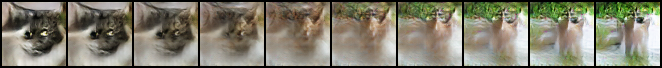
\includegraphics[width=\linewidth]{report_figures/dcgan_interpolation.png}
  \caption{DCGAN interpolation.}
\end{subfigure}

\begin{subfigure}{0.9\linewidth}
  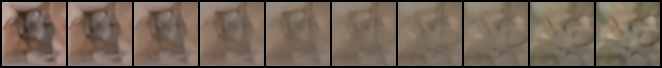
\includegraphics[width=\linewidth]{report_figures/vae_interpolation.png}
  \caption{VAE interpolation.}
\end{subfigure}

\begin{subfigure}{0.9\linewidth}
  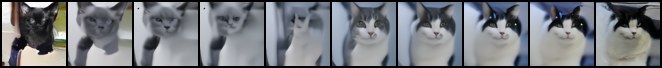
\includegraphics[width=\linewidth]{report_figures/ddpm_interpolation.png}
  \caption{DDPM interpolation.}
\end{subfigure}
\caption{Latent/noise interpolations for the best cat-only models.}
\label{fig:interpolation}
\end{figure}

The DDPM interpolation gives the most convincing semantic transition.
The generated samples change gradually from one cat-like image to another, while most intermediate images remain realistic and recognisable as cats.
This smoothness is important because it shows that small changes in the input lead to gradual and meaningful changes in the generated image.
It suggests that the deterministic DDPM sampler behaves smoothly along the chosen noise interpolation path instead of producing only disconnected realistic samples.
The DCGAN interpolation is partly continuous between neighbouring samples, but the transition is less stable because some middle images lose realistic cat structure.
The VAE interpolation changes smoothly in colour and overall shape, but the outputs remain blurry and contain less visual detail.
These results show different strengths and weaknesses of the models.
DDPM gives the best balance between smooth transition and realistic image structure.
DCGAN can produce sharper images, but its interpolation is less reliable.
VAE gives a smooth transition, but the blur shows that smoothness alone does not guarantee high image quality.

\section{Cats-and-dogs extension}

The best cat-only hyperparameters were reused on the mixed cats-and-dogs dataset.
The goal was exploratory: the models were unconditional, so no class label told the generator whether it should produce a cat or a dog.
The mixed-data runs were evaluated with FID against the mixed cats-and-dogs training distribution, not against the cat-only dataset.
This metric measures how well the generated distribution matches the combined animal dataset. It does not determine whether the model has learned clean class-separated cat and dog modes, nor whether each sample is unambiguously a cat or a dog.

DCGAN and VAE use 5000 generated images for this extension. DDPM uses 2500 generated images because of sampling cost.

\begin{table}[H]
\centering
\caption{FID results for the exploratory cats-and-dogs extension.}
\label{tab:catdog-fid}
\begin{tabular}{llr}
\toprule
Method & Evaluation setting & FID \\
\midrule
DCGAN & mixed cats-and-dogs data & 131.02 \\
VAE & mixed cats-and-dogs data, temp. 0.65 & 246.27 \\
DDPM & mixed cats-and-dogs data & \textbf{74.23} \\
\bottomrule
\end{tabular}
\end{table}

\begin{figure}[H]
\centering
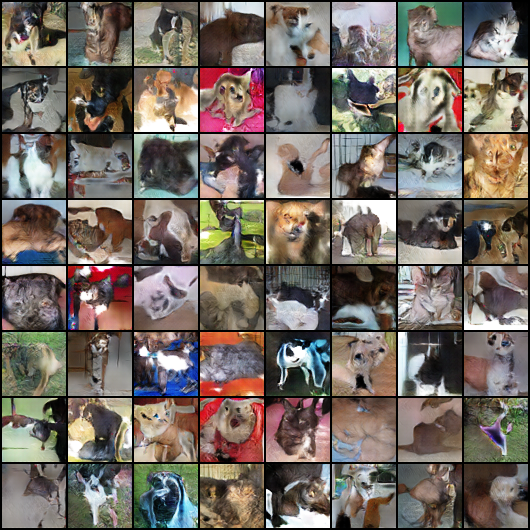
\includegraphics[width=0.72\linewidth]{report_figures/catdog_dcgan_samples.png}
\caption{Exploratory DCGAN generations from the mixed cats-and-dogs dataset.}
\label{fig:catdog}
\end{figure}

\begin{figure}[H]
\centering
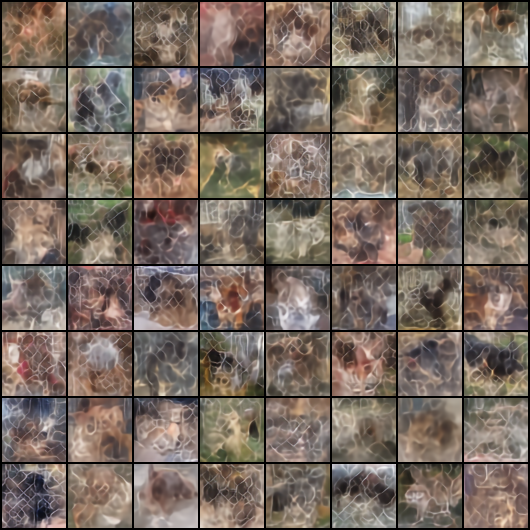
\includegraphics[width=0.72\linewidth]{report_figures/catdog_vae_samples.png}
\caption{Exploratory VAE generations from the mixed cats-and-dogs dataset.}
\end{figure}

\begin{figure}[H]
\centering
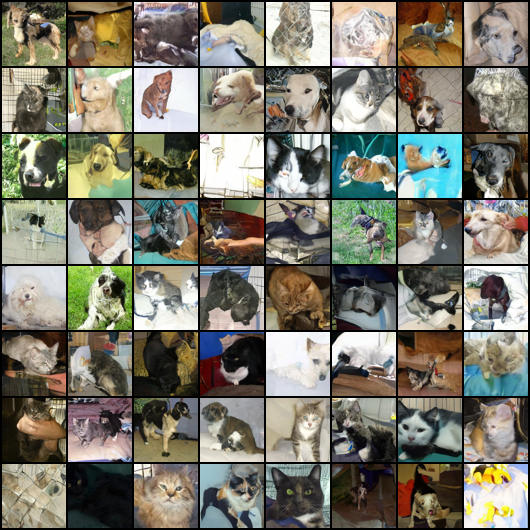
\includegraphics[width=0.72\linewidth]{report_figures/catdog_ddpm_samples.png}
\caption{Exploratory DDPM generations from the mixed cats-and-dogs dataset.}
\end{figure}


Qualitatively, the mixed-data DCGAN and DDPM generate both cat-like and dog-like images, and some samples combine ambiguous animal features.
The VAE again produces mostly blurred, texture-dominated images with only occasional animal-like cues.
This is expected for unconditional generation: without labels or conditioning, the model must represent both classes in a shared distribution.
Class-distinct generation would likely require a conditional model or explicit class labels.

\section{Working with limited computing resources}

The project used several practical decisions to keep training feasible:
\begin{itemize}
  \item all images were resized to $64\times64$,
  \item only compact architectures were trained from scratch,
  \item DDPM FID used 2500 generated samples instead of 5000 because sampling is iterative,
  \item hyperparameter sweeps changed a small number of factors at a time,
  \item checkpoints were saved regularly so interrupted runs could be resumed.
\end{itemize}

\clearpage
\section{Conclusions}

Within this limited-compute experiment, the selected DDPM was the strongest model.
It achieved the best reported FID, the best diversity diagnostics, and the most convincing qualitative samples.
Since DDPM FID was computed with fewer generated images to reduce sampling cost, the exact cross-model FID margin should be interpreted cautiously, but the qualitative evidence supports the same ranking.
The DCGAN was faster to sample and produced sharper images than the VAE, but it was less stable and often created distorted cats.
The VAE was the easiest to train and gave meaningful reconstructions, but random samples were blurry and had the worst FID among the selected final models.

The hyperparameter study also showed that the evaluation criterion matters.
For example, the VAE can reconstruct real cats reasonably well while still sampling poorly from the prior.
The cats-and-dogs extension showed a similar ranking of methods, but it also showed the expected ambiguity of unconditional generation on a mixed animal distribution.
Overall, the wider DDPM was the best practical model for this project.
The best lightweight alternative was the DCGAN variant with a stronger discriminator learning rate.

\section{How to use the code and reproduce the experiments}

All commands below assume that they are executed from the project root directory.
The implementation is organised around YAML configuration files in \texttt{configs/}, training scripts in \texttt{src/}, and convenience experiment runners in \texttt{scripts/}.
Every training run writes checkpoints to \texttt{outputs/checkpoints/<run\_name>/}, sample grids to \texttt{outputs/samples/<run\_name>/}, and a copy of the configuration to \texttt{outputs/checkpoints/<run\_name>/config.yaml}.

\subsection{Environment setup}

\begin{verbatim}
cd /home/sebas/projects/generative-models
python -m venv venv
source venv/bin/activate
pip install -r requirements.txt
\end{verbatim}

The expected dataset folders are:
\begin{verbatim}
data/raw/cats
data/raw/catdog
\end{verbatim}
If the data is moved, the corresponding \texttt{dataset\_root} value in each YAML config should be changed.

\subsection{Training individual models}

Individual models can be trained with:
\begin{verbatim}
./venv/bin/python -m src.train_dcgan \
  --config configs/<selected-dcgan-config>.yaml --device cuda

./venv/bin/python -m src.train_vae \
  --config configs/<selected-vae-config>.yaml --device cuda

./venv/bin/python -m src.train_ddpm \
  --config configs/<selected-ddpm-config>.yaml --device cuda
\end{verbatim}

Training can be resumed from the latest training checkpoint by adding \texttt{--resume}.
For example:
\begin{verbatim}
./venv/bin/python -m src.train_ddpm \
  --config configs/<selected-ddpm-config>.yaml \
  --resume outputs/checkpoints/<selected-ddpm-run>/training_latest.pt \
  --device cuda
\end{verbatim}

\subsection{Running the hyperparameter sweeps}

The full experiment sweeps are launched with:
\begin{verbatim}
PYTHON_BIN=./venv/bin/python \
  bash scripts/run_dcgan_experiments.sh --device cuda
PYTHON_BIN=./venv/bin/python \
  bash scripts/run_vae_experiments.sh --device cuda
PYTHON_BIN=./venv/bin/python \
  bash scripts/run_ddpm_experiments.sh --device cuda
\end{verbatim}

For a short smoke test, the number of epochs can be overridden:
\begin{verbatim}
PYTHON_BIN=./venv/bin/python \
  bash scripts/run_dcgan_experiments.sh --epochs 30 --device cuda
\end{verbatim}

The cats-and-dogs extension for the three best model configurations is launched with:
\begin{verbatim}
PYTHON_BIN=./venv/bin/python \
  bash scripts/run_catdog_best_models.sh --device cuda
\end{verbatim}
If interrupted, it can be resumed with:
\begin{verbatim}
RESUME=1 PYTHON_BIN=./venv/bin/python \
  bash scripts/run_catdog_best_models.sh --device cuda
\end{verbatim}

\subsection{Generating evaluation artefacts}

FID for all latest experiment checkpoints was computed with:
\begin{verbatim}
PYTHON_BIN=./venv/bin/python \
  bash scripts/run_latest_fid_experiments.sh --device cuda
\end{verbatim}
This evaluates DCGAN and VAE with 5000 generated images and DDPM with 2500 generated images.
The script also evaluates several VAE sampling temperatures and writes a summary CSV to \texttt{outputs/fid/}.

The final sample grids were generated with:
\begin{verbatim}
./venv/bin/python -m src.generate \
  --model dcgan \
  --checkpoint outputs/checkpoints/<selected-dcgan-run>/generator_latest.pt \
  --config configs/<selected-dcgan-config>.yaml \
  --num-images 64 --batch-size 64 \
  --out-dir outputs/generated/<dcgan-grid-dir> \
  --device cuda

./venv/bin/python -m src.generate \
  --model vae \
  --checkpoint outputs/checkpoints/<selected-vae-run>/model_latest.pt \
  --config configs/<selected-vae-config>.yaml \
  --num-images 64 --batch-size 64 \
  --sample-temperature 0.65 \
  --out-dir outputs/generated/<vae-grid-dir> \
  --device cuda

./venv/bin/python -m src.generate \
  --model ddpm \
  --checkpoint outputs/checkpoints/<selected-ddpm-run>/model_latest.pt \
  --config configs/<selected-ddpm-config>.yaml \
  --num-images 64 --batch-size 8 \
  --out-dir outputs/generated/<ddpm-grid-dir> \
  --device cuda
\end{verbatim}

The VAE reconstruction grid was generated with:
\begin{verbatim}
./venv/bin/python -m src.reconstruct_vae \
  --checkpoint outputs/checkpoints/<selected-vae-run>/model_latest.pt \
  --config configs/<selected-vae-config>.yaml \
  --num-images 64 --batch-size 64 --num-workers 8 \
  --out-dir outputs/reconstructions/<vae-reconstruction-dir> \
  --device cuda
\end{verbatim}

Diversity diagnostics for the final models were generated with:
\begin{verbatim}
./venv/bin/python -m src.diversity \
  --model dcgan \
  --checkpoint outputs/checkpoints/<selected-dcgan-run>/generator_latest.pt \
  --config configs/<selected-dcgan-config>.yaml \
  --num-images 256 --batch-size 64 --device cuda

./venv/bin/python -m src.diversity \
  --model vae \
  --checkpoint outputs/checkpoints/<selected-vae-run>/model_latest.pt \
  --config configs/<selected-vae-config>.yaml \
  --num-images 256 --batch-size 64 \
  --sample-temperature 0.65 --device cuda

./venv/bin/python -m src.diversity \
  --model ddpm \
  --checkpoint outputs/checkpoints/<selected-ddpm-run>/model_latest.pt \
  --config configs/<selected-ddpm-config>.yaml \
  --num-images 64 --batch-size 8 --device cuda
\end{verbatim}

The interpolation grids were generated with:
\begin{verbatim}
./venv/bin/python -m src.interpolate \
  --model dcgan \
  --checkpoint outputs/checkpoints/<selected-dcgan-run>/generator_latest.pt \
  --config configs/<selected-dcgan-config>.yaml \
  --steps 10 --seed 112 \
  --out-dir outputs/interpolations/<dcgan-interpolation-dir> \
  --device cuda

./venv/bin/python -m src.interpolate \
  --model vae \
  --checkpoint outputs/checkpoints/<selected-vae-run>/model_latest.pt \
  --config configs/<selected-vae-config>.yaml \
  --steps 10 --seed 720 --sample-temperature 0.65 \
  --out-dir outputs/interpolations/<vae-interpolation-dir> \
  --device cuda

./venv/bin/python -m src.interpolate \
  --model ddpm \
  --checkpoint outputs/checkpoints/<selected-ddpm-run>/model_latest.pt \
  --config configs/<selected-ddpm-config>.yaml \
  --steps 10 --seed 360 \
  --out-dir outputs/interpolations/<ddpm-interpolation-dir> \
  --device cuda
\end{verbatim}

\subsection{Reproducibility notes}

The YAML configs contain fixed seeds, and the scripts call a shared seed-setting utility for Python, NumPy, and PyTorch.
This makes the experiments reproducible in practice, but exact bitwise equality is not guaranteed on GPU because some CUDA kernels can be nondeterministic.
For reproducible comparison, the same config, checkpoint, sample count, VAE temperature, and device setting should be reported.
FID values should only be compared directly when the number of generated images is the same. In this report, comparisons inside DCGAN and VAE use 5000 samples, while comparisons inside DDPM use 2500 samples. Therefore, the final cross-family ranking should be understood as a combined FID-and-visual-inspection judgement rather than a perfectly sample-count-controlled FID comparison.

\section{Use of Generative AI in the Project}

Generative AI tools, such as ChatGPT, were used throughout the project as supportive instruments.
They assisted in code optimisation, improving code readability, and supporting the implementation of selected methods.
In the preparation of this report, generative AI was used to support theoretical explanations and as a tool for text refinement and editing.
All generated content was reviewed and adapted to ensure correctness and consistency with the project objectives.

\begin{thebibliography}{99}

\bibitem{catdataset}
W. Zhang, J. Sun, and X. Tang, ``Cat Head Detection --- How to Effectively Exploit Shape and Texture Features,'' in \textit{Proc. ECCV}, 2008. Dataset: \url{https://www.kaggle.com/datasets/crawford/cat-dataset}.

\bibitem{kingma2014vae}
D.~P. Kingma and M. Welling, ``Auto-Encoding Variational Bayes,'' in \textit{Proc. ICLR}, 2014.

\bibitem{higgins2017betavae}
I. Higgins, L. Matthey, A. Pal, C. Burgess, X. Glorot, M. Botvinick, S. Mohamed, and A. Lerchner, ``$\beta$-VAE: Learning Basic Visual Concepts with a Constrained Variational Framework,'' in \textit{Proc. ICLR}, 2017.

\bibitem{goodfellow2014gan}
I.~J. Goodfellow, J. Pouget-Abadie, M. Mirza, B. Xu, D. Warde-Farley, S. Ozair, A. Courville, and Y. Bengio, ``Generative Adversarial Nets,'' in \textit{Proc. NeurIPS}, 2014.

\bibitem{sohldickstein2015}
J. Sohl-Dickstein, E.~A. Weiss, N. Maheswaranathan, and S. Ganguli, ``Deep Unsupervised Learning using Nonequilibrium Thermodynamics,'' in \textit{Proc. ICML}, 2015.

\bibitem{ho2020ddpm}
J. Ho, A. Jain, and P. Abbeel, ``Denoising Diffusion Probabilistic Models,'' in \textit{Proc. NeurIPS}, 2020.

\bibitem{nichol2021improved}
A. Nichol and P. Dhariwal, ``Improved Denoising Diffusion Probabilistic Models,'' in \textit{Proc. ICML}, 2021.

\bibitem{dhariwal2021beatsgans}
P. Dhariwal and A. Nichol, ``Diffusion Models Beat GANs on Image Synthesis,'' in \textit{Proc. NeurIPS}, 2021.

\bibitem{song2021ddim}
J. Song, C. Meng, and S. Ermon, ``Denoising Diffusion Implicit Models,'' in \textit{Proc. ICLR}, 2021.

\bibitem{rombach2022ldm}
R. Rombach, A. Blattmann, D. Lorenz, P. Esser, and B. Ommer, ``High-Resolution Image Synthesis with Latent Diffusion Models,'' in \textit{Proc. CVPR}, 2022.

\bibitem{radford2016dcgan}
A. Radford, L. Metz, and S. Chintala, ``Unsupervised Representation Learning with Deep Convolutional Generative Adversarial Networks,'' in \textit{Proc. ICLR}, 2016.

\bibitem{miyato2018spectralnorm}
T. Miyato, T. Kataoka, M. Koyama, and Y. Yoshida, ``Spectral Normalization for Generative Adversarial Networks,'' in \textit{Proc. ICLR}, 2018.

\bibitem{arjovsky2017wgan}
M. Arjovsky, S. Chintala, and L. Bottou, ``Wasserstein Generative Adversarial Networks,'' in \textit{Proc. ICML}, 2017.

\bibitem{gulrajani2017wgangp}
I. Gulrajani, F. Ahmed, M. Arjovsky, V. Dumoulin, and A.~C. Courville, ``Improved Training of Wasserstein GANs,'' in \textit{Proc. NeurIPS}, 2017.

\bibitem{salimans2016improved}
T. Salimans, I. Goodfellow, W. Zaremba, V. Cheung, A. Radford, and X. Chen, ``Improved Techniques for Training GANs,'' in \textit{Proc. NeurIPS}, 2016.

\bibitem{karras2018progan}
T. Karras, T. Aila, S. Laine, and J. Lehtinen, ``Progressive Growing of GANs for Improved Quality, Stability, and Variation,'' in \textit{Proc. ICLR}, 2018.

\bibitem{karras2020stylegan2}
T. Karras, S. Laine, M. Aittala, J. Hellsten, J. Lehtinen, and T. Aila, ``Analyzing and Improving the Image Quality of StyleGAN,'' in \textit{Proc. CVPR}, 2020.

\bibitem{karras2020ada}
T. Karras, M. Aittala, J. Hellsten, S. Laine, J. Lehtinen, and T. Aila, ``Training Generative Adversarial Networks with Limited Data,'' in \textit{Proc. NeurIPS}, 2020.

\bibitem{vandenoord2017vqvae}
A. van den Oord, O. Vinyals, and K. Kavukcuoglu, ``Neural Discrete Representation Learning (VQ-VAE),'' in \textit{Proc. NeurIPS}, 2017.

\bibitem{razavi2019vqvae2}
A. Razavi, A. van den Oord, and O. Vinyals, ``Generating Diverse High-Fidelity Images with VQ-VAE-2,'' in \textit{Proc. NeurIPS}, 2019.

\bibitem{heusel2017fid}
M. Heusel, H. Ramsauer, T. Unterthiner, B. Nessler, and S. Hochreiter, ``GANs Trained by a Two Time-Scale Update Rule Converge to a Local Nash Equilibrium,'' in \textit{Proc. NeurIPS}, 2017.

\bibitem{dogsvscats}
Kaggle, ``Dogs vs.\ Cats,'' \url{https://www.kaggle.com/competitions/dogs-vs-cats/}.

\end{thebibliography}

\clearpage
\appendix
\section{Detailed VAE temperature results}
\label{app:vae-full-results}

Table \ref{tab:vae-full-temperature} reports the complete VAE temperature sweep used to produce Tables \ref{tab:vae-hparam} and \ref{tab:vae-temp-summary}.
All values are FID scores computed with 5000 generated images. Lower values are better.

\begin{table}[H]
\centering
\small
\caption{Full VAE FID results for each tested sampling temperature.}
\label{tab:vae-full-temperature}
\resizebox{\linewidth}{!}{%
\begin{tabular}{llrrrr}
\toprule
Variant & Main change & Temp. 0.50 & Temp. 0.65 & Temp. 0.80 & Best temp. \\
\midrule
Baseline & reference setting & 248.30 & 241.81 & 248.07 & 0.65 \\
Prior-matching variant & stronger prior matching & 189.33 & 200.92 & 227.40 & 0.50 \\
$\beta=0.25$ & intermediate KL regularisation & 191.54 & 197.92 & 227.32 & 0.50 \\
$\beta=0.5$ & stronger KL regularisation & 188.23 & \textbf{176.68} & 199.93 & 0.65 \\
Latent dimension 256 & smaller latent space & 227.07 & 226.71 & 241.70 & 0.65 \\
Latent dimension 512 & larger latent space & 236.34 & 224.25 & 236.60 & 0.65 \\
Extra decoder refinement & extra decoder refine block & 193.75 & 196.83 & 227.12 & 0.50 \\
No multiscale loss & single-scale reconstruction & 199.47 & 214.01 & 239.79 & 0.50 \\
\bottomrule
\end{tabular}
}
\end{table}

\end{document}
